%%%%%%%%%%%%%%%%%%%%%%%%%%%%%%%%%%%%%%%%%%%%%%%%%%%%%%%%%%%%%%%%%%%%%%%%%%%%%%%%%%
%%																				%%
%% File name: 		10max.tex													%%
%% Project name:	Hochleistungsantenne										%%
%% Type of work:	T3X00 project work											%%
%% Author:			Sarah Brückner, Maximilian Stiefel, Hannes Bohnengel		%%
%% Date:			27th Arpil 2016												%%
%% University:		DHBW Ravensburg Campus Friedrichshafen						%%
%% Comments:		Created in gedit with tab width = 4							%%
%%																				%%
%%%%%%%%%%%%%%%%%%%%%%%%%%%%%%%%%%%%%%%%%%%%%%%%%%%%%%%%%%%%%%%%%%%%%%%%%%%%%%%%%%

\chapter{Hintergründe}

\section{Bahnmechanik}

\subsection{Die Keplerschen Gesetze}
Seit der Antike galt die Erklärung der Bewegung der Planeten und die Vorhersage dieser als eine große Herausforderung. Theorien von Ptolemaios mit seinem geozentrischen Weltbild und Kopernikus mit seinem heliozentrischen Weltbild führten bereits im 16. Jahrhundert zu brauchbaren Modellen zur Vorhersage der Planetenbewegungen. Diese Modelle unterlagen jedoch Ungenauigkeiten, „die in mit Instrumenten des 16. Jahrhunderts bereits messbaren Breichen lagen“ (siehe S. 20 in \cite{Raumflugm}). 
%%%%%%%%%%%%%%%%%%%%%%%%%%%%%%%%%%%%%%%%%%%%%%%%%%%%%%%%%%%%%%%%%%%%%%%%%%%%%%%%%%%%%%%%%%%%%%
\begin{figure}[h]                                                                       %%
	\centering                                                                            	%%
	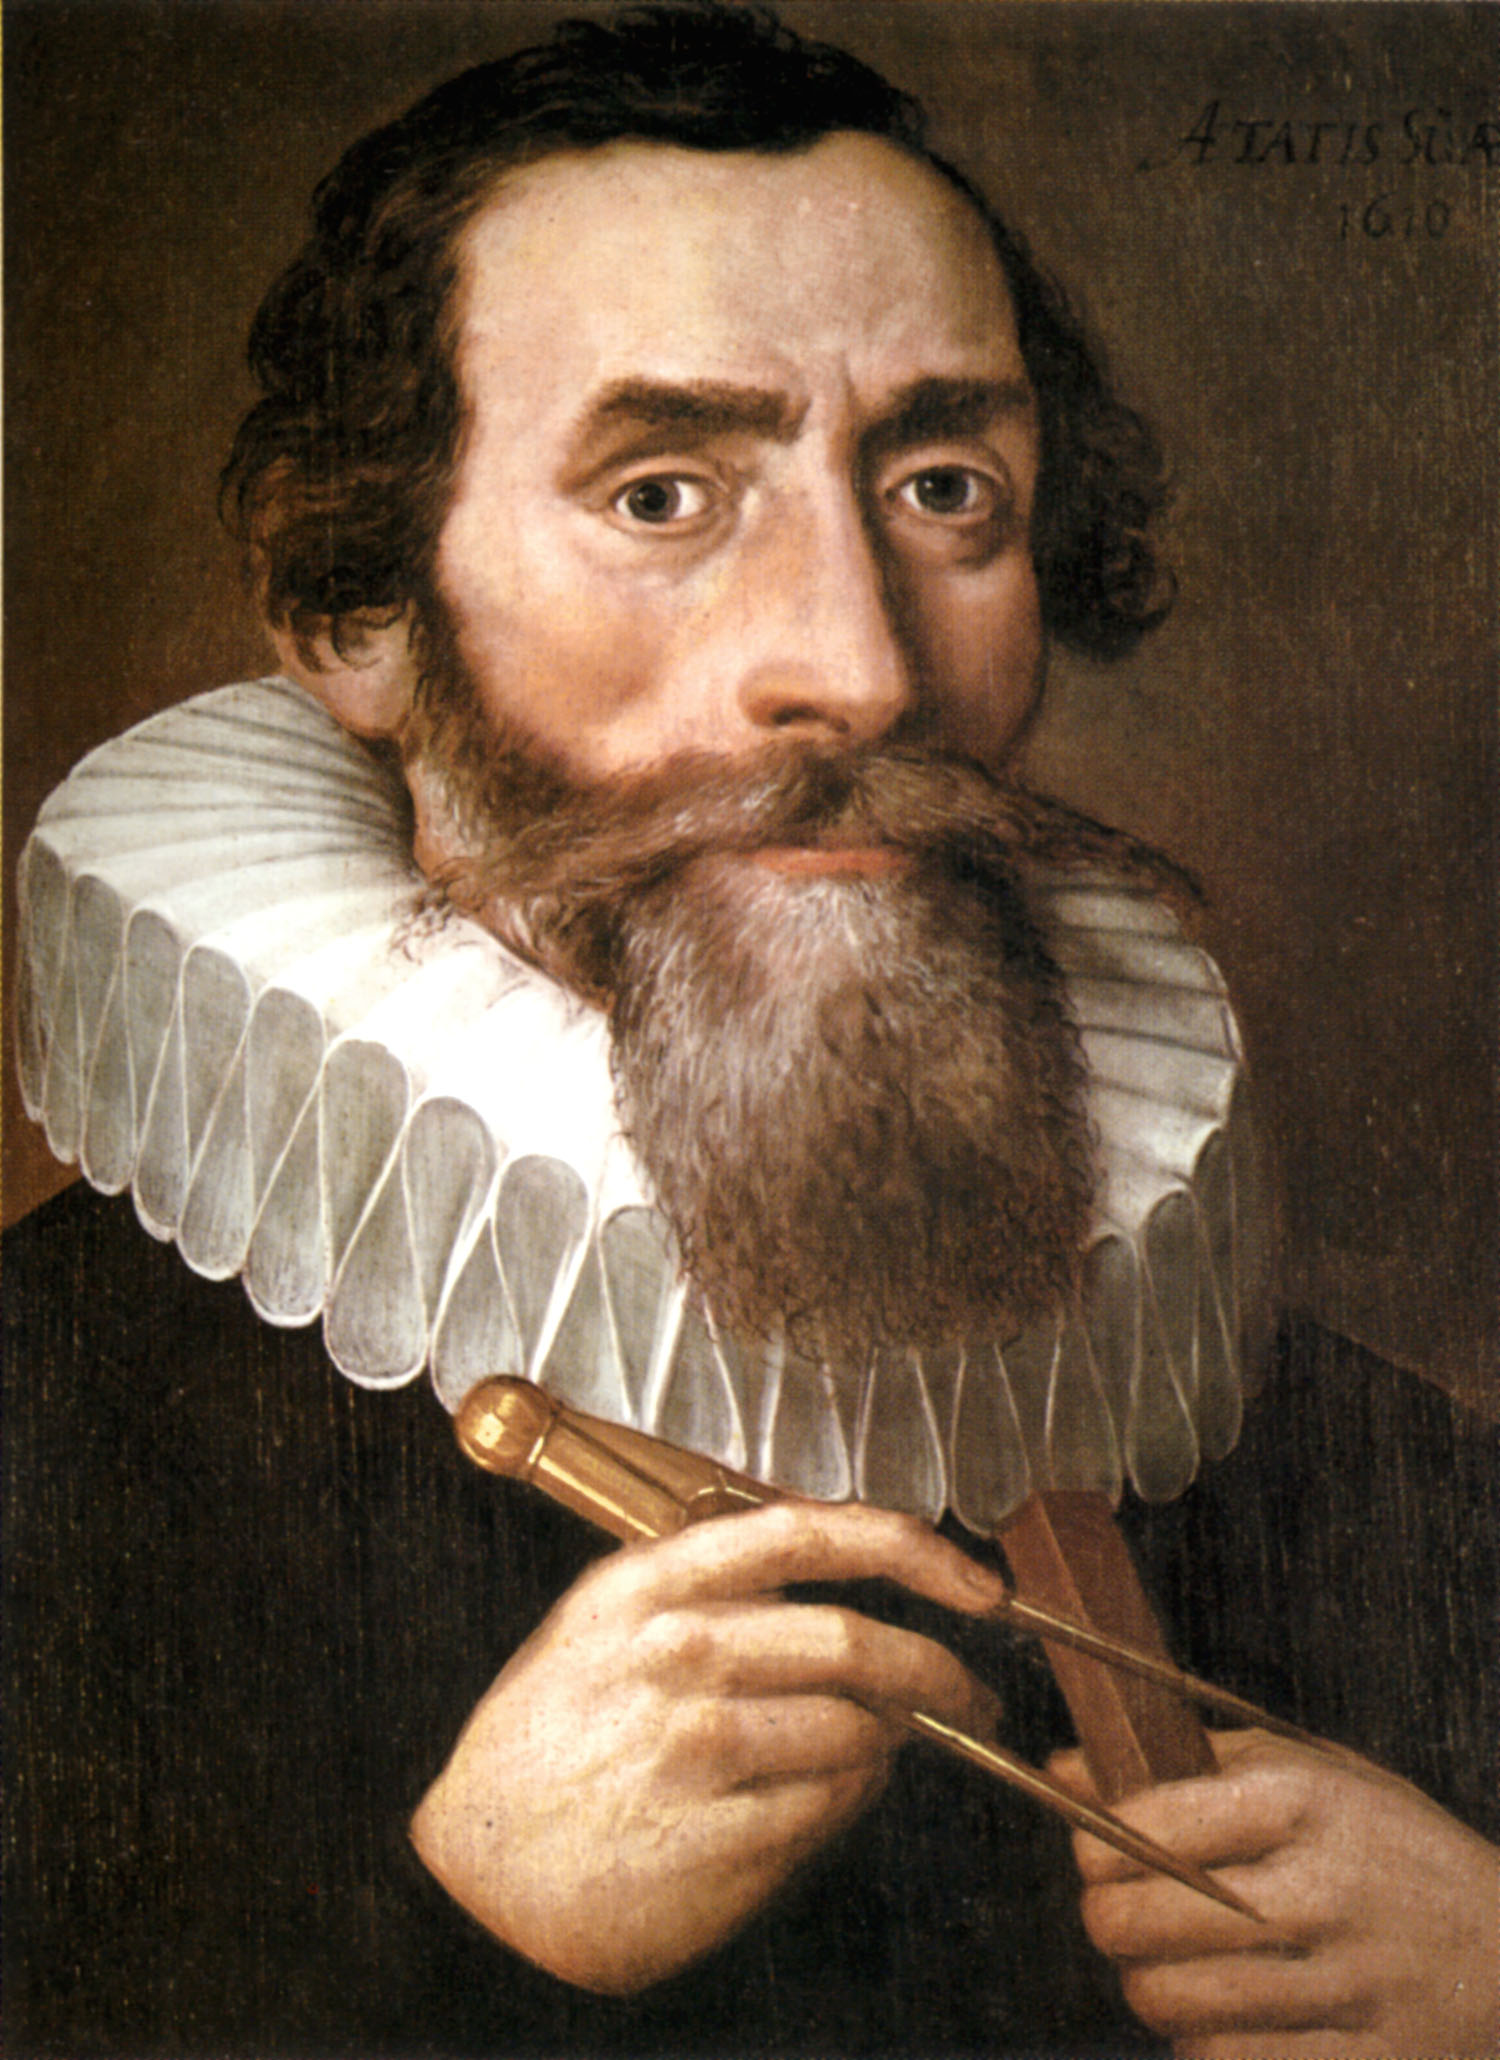
\includegraphics[width=0.3\textwidth]{./images/kepler.jpg}                        %%
	\caption[Bahnelemente]{Johannes Kepler (1571-1630), Quelle: \cite{Wiki:Kepler}}                        %%
	\label{fig:bahnelemente}                                                                %%
\end{figure}                                                                              	%%
%%%%%%%%%%%%%%%%%%%%%%%%%%%%%%%%%%%%%%%%%%%%%%%%%%%%%%%%%%%%%%%%%%%%%%%%%%%%%%%%%%%%%%%%%%%%%% 
Der mathematische Aufwand hinter diesen Modellen war enorm. Selbst das kopernikanische Weltbild, dass einige Vereinfachnugen mit sich brachte, bediente sich der Überlagerung einer Vielzahl von Kreisbwegungen, um das Verhalten der Planeten zu erklären. Resignierend zog sich zu der Zeit die katholische Kirsche und mit ihr viele Gelehrte auf den Standpunkt zurück, dass „die Frage, welche der Theorien die korrekte sei, [...] schlicht unbeantwortbar“ wäre (siehe S. 21 in \cite{Raumflugm}). 
\newpar
Ein deutscher Mathematiker und Astronom, Johannes Kepler, war hier anderer Auffassung. Er war überzeugter Kopernikaniker und stand im Dienste des Kaisers Rudolph II. Schließlich gelang es ihm aus seinen Beobachtungen drei einfache Gesetze herzuleiten. Seine Gesetze führten zu Vorhersagen der Planetenbewegungen nie da gewesener Präzision, welche er seinem Dienstherr widmend in den Rudolphinischen Tabellen niederschrieb. Steiner und Schlagerl schreiben in Ihrem Buch Raumflugmechanik, dass ohne die Vorarbeit Keplers keine Weltraumtechnik je existiert hätte (vgl. S. 21 in \cite{Raumflugm}). Die drei Gesetze lauten:
\begin{enumerate}
	\item Keplersches Gesetz: Die Planeten umlaufen die Sonne auf elliptischen Bahnen. In einem der Brennpunkte dieser Ellipsen befindet sich die Sonne. 
	\item Keplersches Gesetz: Die Linie von der Sonne zu einem Planeten überstreicht in gleichen Zeiten gleiche Flächen.
	\item Keplersches Gesetz: Die Quadrate der Umlaufzeiten zweier Planeten verhalten sich zueinander so wie die Kuben der großen Halbachsen ihrer Bahnellipsen. 
\end{enumerate}   
Kepler starb 1630 und damit 12 Jahre vor Newtons Geburt. Mit seinen Werken hinterlies Kepler Newton alles, um das Gravitationsgesetz später herleiten zu können. 
\subsection{Die Bahnelemente}
%%%%%%%%%%%%%%%%%%%%%%%%%%%%%%%%%%%%%%%%%%%%%%%%%%%%%%%%%%%%%%%%%%%%%%%%%%%%%%%%%%%%%%%%%%%%%%
\begin{figure}[!htbp]                                                                       %%
	\centering                                                                            	%%
	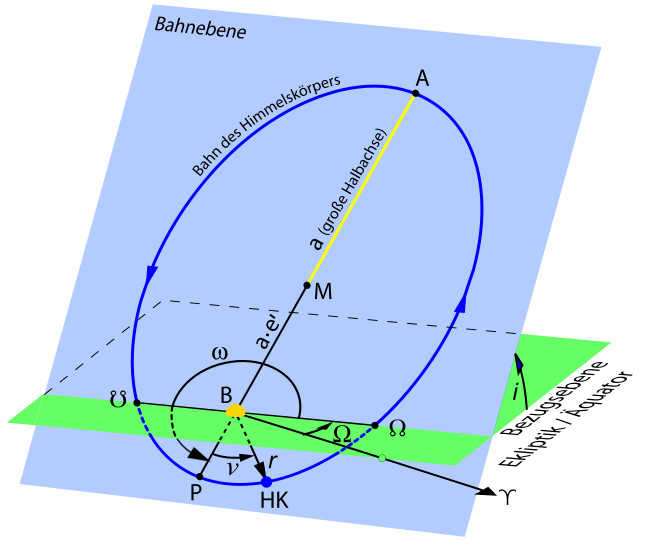
\includegraphics[width=0.8\textwidth]{./images/bahnelemente.jpg}                        %%
	\caption[Bahnelemente]{Bahnelemente, Quelle: \cite{Wiki:Bahnel}}                        %%
	\label{fig:bahnelemente}                                                                %%
\end{figure}                                                                              	%%
%%%%%%%%%%%%%%%%%%%%%%%%%%%%%%%%%%%%%%%%%%%%%%%%%%%%%%%%%%%%%%%%%%%%%%%%%%%%%%%%%%%%%%%%%%%%%%   
Die Bahnelemente dienen der Beschreibung einer Bewegung eines Himmelskörpers auf einer Umlaufbahn (meist einer Ellipse). Dieser Körper unterliegt den Keplerschen Gesetzen. Wird die Bewegung eines Himmelskörpers durch äußere Einflüsse (z.B. Gravitationskraft der Sonne) nicht gestört, so kann sie durch sechs Größen beschrieben werden. Diese Größen sind die Bahnelemente. Zwei Bahnelemente beschreiben die Form der Bahn, drei legen die Lage der Bahn im dreidimensionalen Raum fest und ein Bahnelement gibt an zu welcher Zeit sich der Himmelskörper wo auf der Bahn befunden hat. 
\\\\Diese Bahnelemente reichen in der Praxis nicht aus, um die Position eines Himmelskörpers z.B. eines Satelliten mit einem Vorhersagemodell berechnen zu können. Aus diesem Grund werden die Bahnelemente meist um von Vorhersagemodellen benötigten Informationen ergänzt.       
Im Folgenden werden die Bahnelemente in Ihrer Bedeutung anhand der Abbildung \ref{fig:bahnelemente} erläutert. 

\subsubsection*{Gestalt der Bahn}
Um die Gestalt der Bahn zu beschreiben wird die \textbf{numerische Exzentrizität e} und die Angabe der Länge der \textbf{großen Halbachse a} benötigt.
\\\\Zunächst soll die Ellipse an sich betrachtet werden. Die einfachste Möglichkeit eine Ellipse zu konstruieren besteht darin zwei Nägel in einer Holzplatte mit einem Stück Schnur mit einer Schlaufe zu verbinden. Das Stück Schnur muss länger sein als der Abstand zwischen beiden Nägeln. Nimmt man nun einen Bleistift und drückt ihn in der Schlaufe gegen die Schnur, kann man die beiden Nägel mit Kontakt der Bleistiftspitze zum Holzbrett umrunden. Hält man die Schnur konstant auf Spannung, so ergibt sich eine Ellipse. Nichts anderes besagt die folgende Mengendefinition mit Bezug zu Abbildung \ref{fig:ellipse}. 
\begin{equation}
E = \{P | \overline{F_{1}P} + \overline{F_{2}P} = 2a = konstant\}
\end{equation}
\ensuremath{F_{1}} und \ensuremath{F_{2}} heißen Brennpunkte der Ellipse. \ensuremath{M} ist der Mittelpunkt der Ellipse. \ensuremath{S_{1}} und \ensuremath{S_{2}} sind die Haupt-, \ensuremath{S_{3}} und \ensuremath{S_{4}} die Nebenscheitel.      
%%%%%%%%%%%%%%%%%%%%%%%%%%%%%%%%%%%%%%%%%%%%%%%%%%%%%%%%%%%%%%%%%%%%%%%%%%%%%%%%%%%%%%%%%%%%%%
\begin{figure}[!htbp]                                                                       %%
	\centering                                                                            	%%
	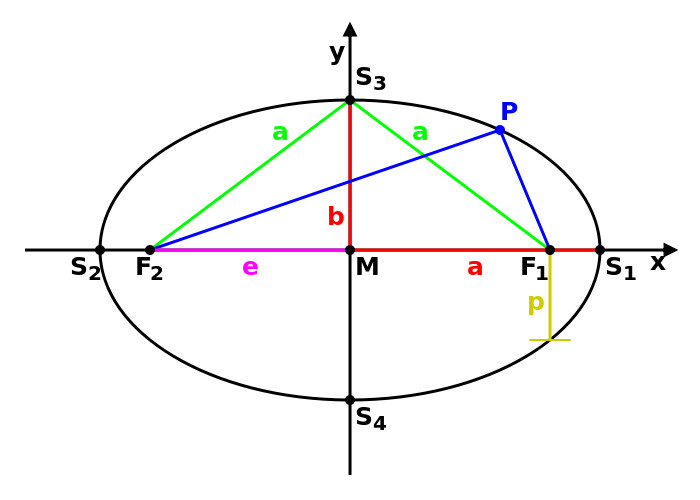
\includegraphics[width=0.6\textwidth]{./images/ellipse.jpg}                             %%
	\caption[Ellipse]{Ellipse, Quelle: Wikipedia}                                           %%
	\label{fig:ellipse}                                                                     %%
\end{figure}                                                                              	%%
%%%%%%%%%%%%%%%%%%%%%%%%%%%%%%%%%%%%%%%%%%%%%%%%%%%%%%%%%%%%%%%%%%%%%%%%%%%%%%%%%%%%%%%%%%%%%%      
Die Strecke \ensuremath{\overline{MS_{1}}} ist gleich der Strecke \ensuremath{\overline{MS_{2}}}. Man spricht bei der Länge dieser Strecke von der großen Halbachse a. Beide Strecken ergeben zusammen die Hauptachse \ensuremath{\overline{S_{1}S_{2}}}. Analog gibt es hierzu die Nebenachse, welche durch die Strecke \ensuremath{\overline{S_{3}S_{4}}} bestimmt wird. Die kleinen Halbachsen sind \ensuremath{\overline{MS_{3}}} und \ensuremath{\overline{MS_{4}}}. Diese haben die Längen b.  Das Wort numerisch gibt bei der Exzentrizität an, dass diese sich auf eine andere Größe (die große Halbachse) bezieht. Der Wert der numerischen Exzentrizität lässt sich in vier Bereiche aufteilen: 
\begin{itemize}
	\item Der Wert 0 repräsentiert eine perfekte kreisförmige Bahn.
	\item Der Bereich von 0 bis 1 beschreibt eine elliptische Bahn.
	\item Der Wert 1 erzeugt eine exakt parabolische Bahn.
	\item Jeder Wert größer 1 gehört zu einer immer offener werdenden Hyperbel.  
\end{itemize}   

Bis zum Wert 1 handelt es sich um eine geschlossene Bahn. Oberhalb von 1 ist die Bahn immer geöffnet. Das bedeutet jeder Punkt der Bahn wird von einem Satellit nur einmal abgeschritten. Für eine elliptische Bahn (\ensuremath{e < 1}) kann aus der Halbachse der Ellipse und der numerischen Exzentrizität ein minimaler (\ensuremath{r_{min}}) und ein maximaler (\ensuremath{r_{max}}) Abstand vom Brennpunkt der Ellipse berechnet werden.     

\subsubsection*{Lage der Bahn}


\subsubsection*{Zeitlicher Bezug}
\begin{itemize}
	
	%\parskip0pt
	\item Unter der \textbf{Inklination (i)} versteht man den Winkel zwischen 
	Bahn- (blau) und Äquatorebene (grün). Der Schnittpunkt mit der Äquatorebene ergibt die
	Konotenlinie. 
	\item \textbf{Die Rektaszension des aufsteigenden Knotens (\ensuremath{\Omega})} ist jener Winkel, der zwischen einer Geraden vom Brennpunkt (B) zum Frühlingspunkt (\ensuremath{\gamma}) und einer Geraden vom Brennpunkt zum aufsteigenden Knoten (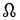
\includegraphics[scale=1.5]{./images/anode.jpg}) ausgebildet wird.  
	\item Die \textbf{Periapsisdistanz \ensuremath{r_{min}}} stellt den Abstand des Perigäums (P) zum Brennpunkt dar. Das Perigäum ist der Punkt auf der Bahn, welcher den geringsten Abstand zum Brennpunkt hat.
	\item \textbf{Apogäum:} Im Gegenzug zu dem Perigäum definiert das Apogäum 
	den größten Erdabstand den der Satellit erreichen kann.
	\item \textbf{Argument des Perigäums:} Unter dem Argument des Perigäum 
	versteht man den Winkel zwischen der Knotenlinie und der Apsidenlinie, welche 
	die beiden Punkte Perigäum mit Apogäum verbindet.
	\item \textbf{Exzentrizität:} Dadurch dass ein Orbit nicht wie ein Kreis 
	beschreiben lässt, wird ein Maß benötigt, welches die Form beschreibt. Die 
	Exzentrizität gibt an, wie weit die beiden Brennpunkte vom Mittelpunkt der 
	Ellipse entfernt sind und beschreibt somit die Form des Orbits.
	\item \textbf{Mittlere Anomalie:} Die Mittlere Anomalie sagt aus, wo sich 
	der Satellit vom Referenzpunkt Perigäum auf seiner Bahn befindet.
	\item \textbf{Große Halbache:} Die Große Halbachse beschreibt die Größe der
	Bahn.
	
\end{itemize}

\subsection{Vorhersagemodelle}

\clearpage